%!TeX program = xelatex

\documentclass[aspectratio=169]{beamer}
\usepackage{fontspec}
\usepackage{graphicx}
\usepackage{xltxtra}
\usepackage[main=russian,english]{babel}

\setmainfont{Iosevka NFM}
\setmonofont{Iosevka NFM}
\setsansfont{Iosevka NFM}
\setromanfont{Iosevka NFM Italic}


\title{sched\_ext}
\author{Шаго Павел Евгеньевич \\[1\baselineskip] Научный руководитель\\ к.ф.-м.н.,
доцент Корхов В. В.}
\institute{Санкт-Петербургский государственный университет \\ Факультет прикладной математики - процессов управления \\ Кафедра моделирования электромеханических и компьютерных систем}

\begin{document}

\begin{frame}
  \titlepage
\end{frame}

\begin{frame}
  \frametitle{Цель и задачи работы}
  \begin{block}{Цель}
    \begin{itemize}
      \item Исследование новой подсистемы планировщика в Linux
    \end{itemize}
  \end{block}

  \begin{block}{Задачи}
    \begin{itemize}
      \item Изучение применимости подсистемы и её реализаций
      \item Составление и вывод результатов из виртуальных окружений (демо)
    \end{itemize}
  \end{block}

\end{frame}

\begin{frame}
  \frametitle{Что такое sched\_ext?}
  sched\_ext -- это инфраструктура позволяющая описывать
  планировщик набором bpf программ (bpf scheduler)
  
  \vspace*{0.3cm}

  1. sched\_ext экспортирует полноценный (необходимый) интерфейс
  планирования, так что любой алгоритм можно реализовать поверх
  этого интерфейса

  2. sched\_ext планировщик можно в любой момент включить или выключить

  3. Целостность системы сохранена вне зависимости от того что делает
  планировщик, в случае ошибок спускаемся до стандартного поведения,
  управление получает EEVDF, а от подсистемы получаем информативную dump трассу
\end{frame}

\begin{frame}
  Преимущества подхода
  \begin{itemize}
      \item Кастомизация под различное поведение
      \item Возможность попробовать различные эвристики
      \item Большая безопасность
      \item Поддержка со стороны крупного бизнеса (Google, Meta')
  \end{itemize} 
  Минусы
  \begin{itemize}
    \item Поддержка только с версии Linux 6.12 (ноябрь 2024)
  \end{itemize}
\end{frame}

\begin{frame}
  \frametitle{Пример: FIFO планировщик с sched-ext}
  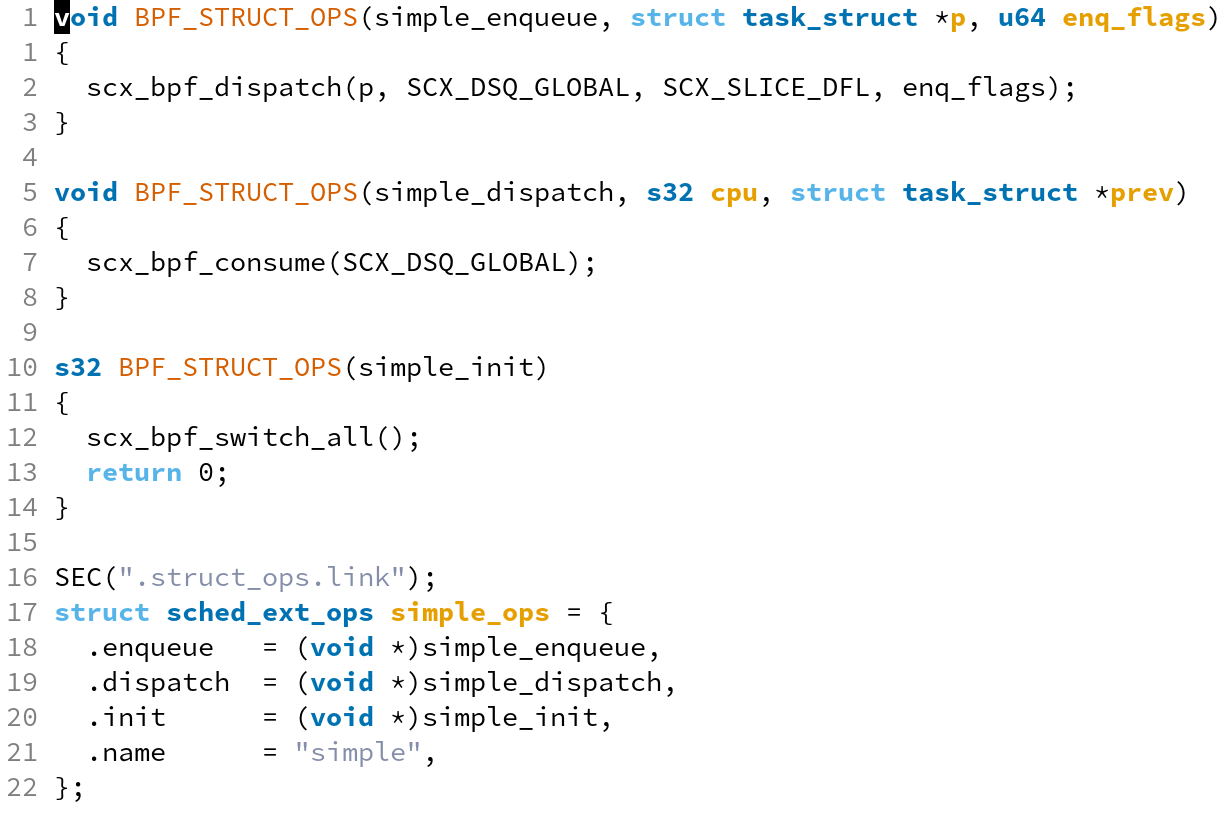
\includegraphics[width=10cm,height=7cm]{res/simple.png}
\end{frame}

\begin{frame}
  \frametitle{NUMA aware (демо 1)}
  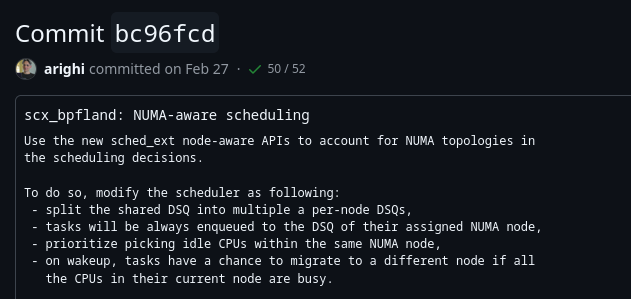
\includegraphics[width=\linewidth]{res/D0_0.png}
\end{frame}

\begin{frame}
  \frametitle{NUMA aware (демо 1)}
  \vspace*{0.2cm}
  \centering
  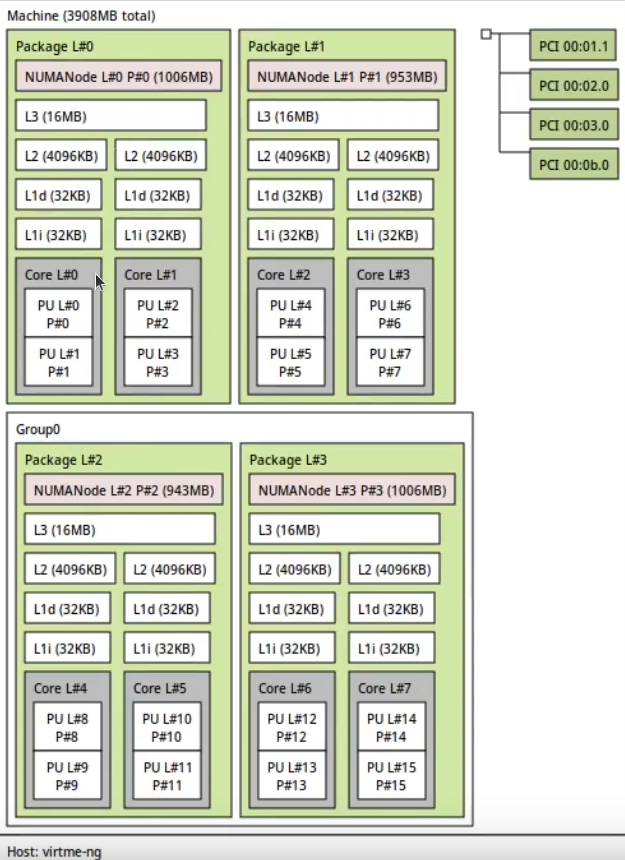
\includegraphics[width=0.7\linewidth]{res/D0_1.png}
\end{frame}

\begin{frame}
  \frametitle{NUMA aware (демо 1)}
  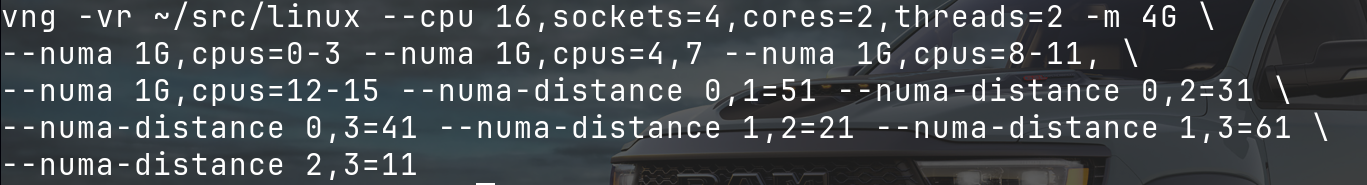
\includegraphics[width=\linewidth]{res/D0_2.png}
  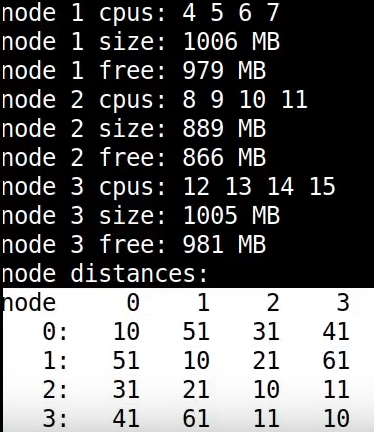
\includegraphics[width=0.3\linewidth]{res/D0_3.png}
  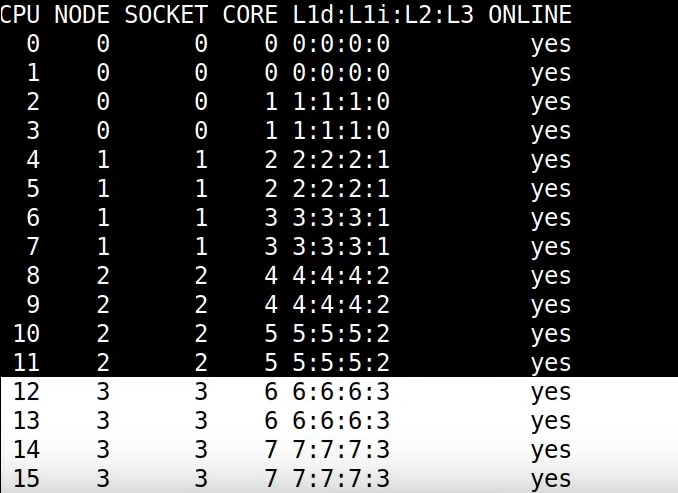
\includegraphics[width=0.47\linewidth]{res/D0_4.png}
\end{frame}

\begin{frame}
  \vspace*{0.2cm}
  \frametitle{NUMA aware (демо 1)}
  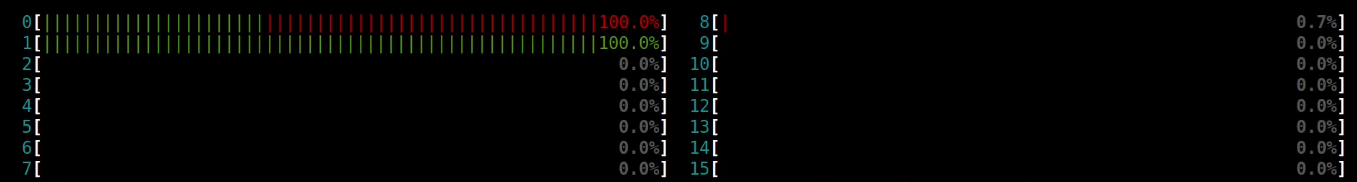
\includegraphics[width=\linewidth]{res/D0_5.png}
  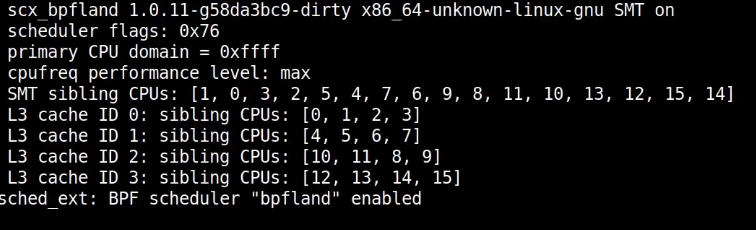
\includegraphics[width=\linewidth]{res/D0_6.png}
  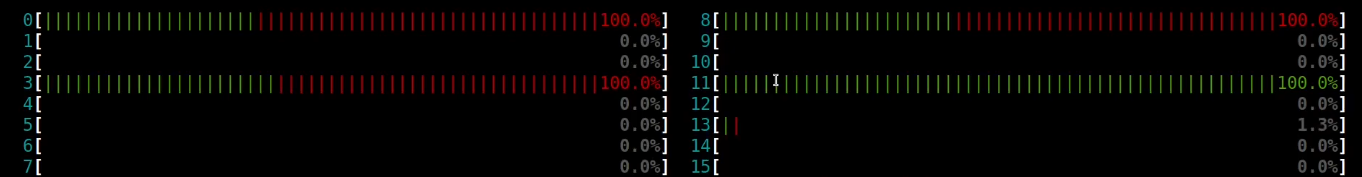
\includegraphics[width=\linewidth]{res/D0_7.png}
\end{frame}

\begin{frame}
  \frametitle{Как уже используется sched\_ext}
  \begin{block}{Цель}
    \begin{itemize}
      \item Оптимизировать производительность продакшн-нагрузок в Meta',
        где ключевой метрикой является 99-й перцентиль задержки ответов.
        Загрузка CPU обычно 40\%, но все равно рассматривается тюнинг
        планировщика.
    \end{itemize}
  \end{block}
  \begin{block}{Основные направления эксперементов}
    \begin{itemize}
      \item Work-conservation – не простаивают ли CPU, когда есть работа?
      \item Idle CPU selection – как правильно выбирать CPU при пробуждении потока?
      \item Soft-affinity – стоит ли закрепить второстепенные задачи за конкретными CPU?
      \item Custom policies – использовать ли разные политики для разных типов потоков?
    \end{itemize}
  \end{block}
\end{frame}

\begin{frame}
  \frametitle{Как уже используется sched\_ext}
  \begin{block}{scx\_simple}
    \begin{itemize}
      \item Поддерживает work-conservation: все CPU делят один dsq
      \item Использует scx\_select\_cpu\_dfl() — отдаёт предпочтение полностью
        свободным ядрам, не стремясь к локальности кешей
      \item Результат: 3.5\% прирост на 1000 машинах
      \item Подтверждено: приоритет полностью свободным ядрам — ключевой фактор прироста
    \end{itemize}
  \end{block}
  \begin{block}{scx\_layered}
    \begin{itemize}
      \item Позволяет разделять потоки на слои с разными политиками
      \item Высокоприоритетные потоки могут прерывать любые другие
      \item В итоге выбран в качестве базы
    \end{itemize}
  \end{block}
\end{frame}

\begin{frame}
  \frametitle{Учет перспективы (демо 2)}
  \vspace*{0.2cm}
  \begin{columns}
    \column{0.5\textwidth}
      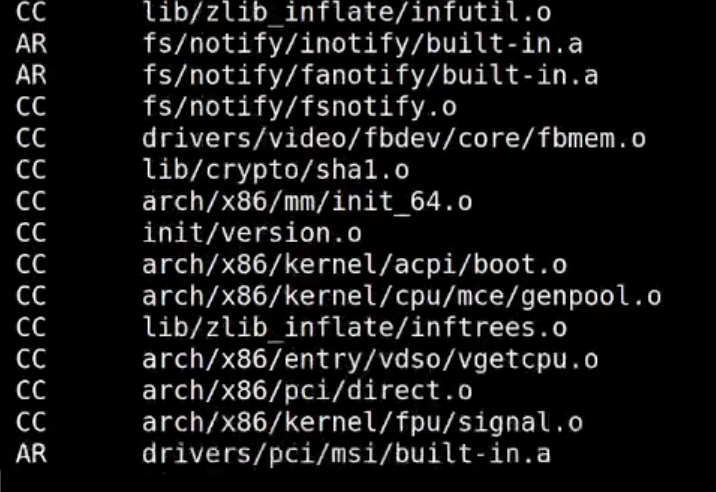
\includegraphics[width=\linewidth]{res/D1_0.png}
    \column{0.5\textwidth}
      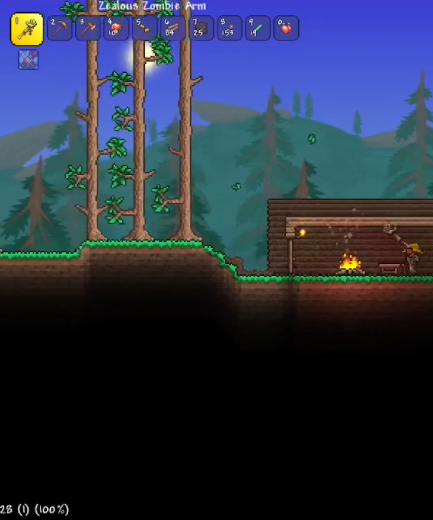
\includegraphics[width=0.85\linewidth]{res/D1_1.png}
  \end{columns}
\end{frame}

\begin{frame}
  \frametitle{Учет перспективы (демо 2)}
  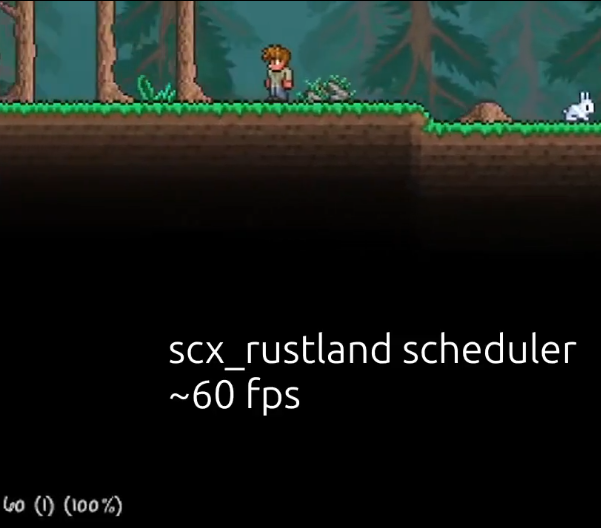
\includegraphics[width=0.5\linewidth]{res/D1_2.png}
\end{frame}

\begin{frame}
  \frametitle{Список использованных источников}

  \begin{thebibliography}{20}

    \bibitem{ari} arighi\_linux

    \bibitem{scx} Исходный код scx, scx\_bpfland \& scx\_rustland
    
    \bibitem{Linux} Исходный код ядра Linux в т. ч. документация к ядру Linux

    \bibitem{LinuxML} Подписка на почтовую рассылку linux-kernel@vger.kernel.org
  
    \bibitem{AndrewT} Andrew S. Tanenbaum, Herbert Bos MODERN OPERATING SYSTEMS Pearson
    Education 2024

  \end{thebibliography}
\end{frame}


\end{document}
